\hsection{The Solution Space}%
\label{sec:solutionSpace}%
%
\hsection{Definitions}%
\label{sec:solutionSpaceDefinitions}%
%
As stated in \autoref{def:optimizationProblemEconomical}, an optimization problem asks us to make a choice between different possible solutions.
We call them \emph{candidate solutions}.
%
\begin{definition}%
\label{def:candidateSolution}%
A \emph{candidate solution}~\solspel\ is one potential solution of an optimization problem.%
\end{definition}%
%
\begin{definition}%
\label{def:solutionSpace}%
The \emph{solution space}~$\solutionSpace$ of an optimization problem is the set of all of its candidate solutions~\solspel.%
\end{definition}%
%
\ruleOfThumb{output1}{The best candidate solution(s) that an optimization algorithm has discovered are (one part) of its \emph{output}.}%
%
Basically, the input of an optimization algorithm is the problem instance~$\instance$ and (one part of) the output would be (at least) one candidate solution~$\solspel\in\solutionSpace$.
This candidate solution is the choice that the optimization process proposes to the human operator.
It therefore holds all the data that the human operator needs to take action, in a form that the human operator can understand, interpret, and execute.
During the optimization process, many such candidate solutions may be created and compared to find and return the best of them.%
%
\endhsection%
%
\hsection{A Programmer's Perspective}%
%
From the programmer's perspective, the solution space is a data structure, e.g., a \codeil{class} in Python.
An instance of this data structure is the candidate solution.
On an abstract level, this data structure could be anything.
It could be a \codeil{list}, a \numpyndarray, a tree data structure, a \codeil{dict}, a graph, a construction plan for a train, anything.

Earlier, I said that we will do a lot of hands-on learning in this optimization book.
We will look at things not \emph{only} from the perspective of an algorithm scientist, but also from the perspective of a \emph{programmer}.
If a programmer is supposed to build algorithms that can deal with arbitrary data structures, she will first think about what kind of operations she will need to perform with them.
In \autoref{lst:Space}, we give an excerpt example of such a \inQuotes{space API.}

\moptipyCode{moptipy/api/space.py}{--labels book --args format}{Space}{An excerpt of an base class for implementing space handlers.}

Now the data structures are basically containers.
\numpyndarrays\ are containers that can be filled with information.
\codeils{list} and \codeils{dict} are such containers as well.
If our algorithms later on should be able to work with arbitrary such container data structures, they will need a way to create them.
\codeil{Space} therefore provides the method \codeil{create}.
They will also need to copy the data from one container to another, for which the \codeil{copy} method is provided.
A data structure instance~\solspel\ is always something that lives in the computer memory.
But we \begin{enumerate*}[label=\emph{\alph*})]%
\item need to show the contents of \solspel\ to a user in a human-readable fashion, because they are the results of the optimization process, and%
\item need to be able to store and load them from files in order to be able to process them with other programs%
\end{enumerate*}.
For this purpose, the methods \codeil{to_str} and \codeil{from_str} are provided.
They convert an instance $\solspel\in\solutionSpace$ to a text string.

By defining the interface \codeil{Space}, we provide a blueprint for the bookkeeping operations that we want to do with the candidate solutions~\solspel.
We can \emph{implement} this interface for all kinds of different solution spaces~\solutionSpace.
This will allow us to basically ignore the exact nature of~\solutionSpace\ in our algorithm implementations.
We can create a variable to hold a~\solspel, we can copy it, and we can read and write it to a file or show its contents to the user.
%
\endhsection%
%
\hsection{Example: Job Shop Scheduling}%
%
What would be a candidate solution to a \gls{JSSP} instance as defined in \autoref{sec:jsspInstance}?
Recall from \autoref{sec:jsspExample} that our goal is to complete the jobs, i.e., the production tasks, as soon as possible.
Hence, a candidate solution should tell us what to do, i.e., how to process the jobs on the machines.%
%
\hsection{Idea: Gantt Chart}%
\label{sec:jssp:gantt}%
%
This is basically what Gantt charts~\cite{W2003GCACA,K2000SORCP} are for.
A Gantt chart defines what each of our~\jsspMachines\ machines has to do at each point in time.
The operations of each job are assigned to time windows on their corresponding machines.
You can find an example illustrated in \autoref{fig:gantt_demo_without_makespan}.

\begin{figure}%
\centering%
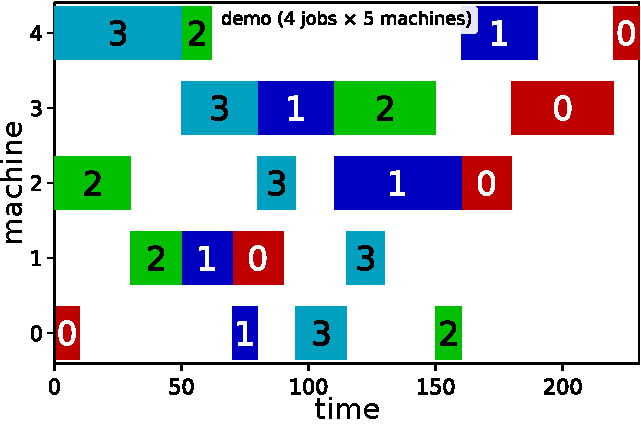
\includegraphics[width=0.7\linewidth]{\currentDir/gantt_demo_without_makespan.pdf}%
\caption{One example candidate solution for the demo instance given in \autoref{fig:jssp_demo_instance}: A Gantt chart assigning a time window to each job on each machine.}%
\label{fig:gantt_demo_without_makespan}%
\end{figure}

The Gantt chart contains one row for each machine.
It is to be read from left to right, where the horizontal axis represents the time units that have passed since the beginning of the job processing.
Each colored bar in the row of a given machine stands for a job and denotes the time window during which the job is processed.
The bar representing operation~\jsspMachineIndex\ of job~\jsspJobIndex\ is painted in the row of machine~\jsspOperationMachine{\jsspJobIndex}{\jsspMachineIndex} and its length equals the time requirement~\jsspOperationTime{\jsspJobIndex}{\jsspMachineIndex}.

\autoref{fig:gantt_demo_without_makespan} illustrates one example solution of our \instStyle{demo} instance as such a Gantt chart.
We use a distinct color for each job.
This chart defines that job~0 starts at time unit~0 on machine~0 and is processed there for ten time units.
Then the machine idles until the 70\textsuperscript{th} time unit, at which point it begins to process job~1 for another ten time units.
After 15~more time units of idling, job~3 will arrive and be processed for 20~time units.
Finally, machine~0 works on job~2 (coming from machine~3) for ten time units starting at time unit~150.

Machine~1 starts its day with an idle period until job~2 arrives from machine~2 at time unit~30 and is processed for 20~time units.
It then processes jobs~1 and~0 consecutively and finishes with job~3 after another idle period.
And so on.

If we wanted to create a Python \codeil{class} to represent the complete information from a Gantt diagram, it could look like \autoref{lst:jssp_gantt}.
Here, we again just subclass \numpyndarray\ to store all data as three-dimensional array.
The array has one row for each of the \jsspMachines~machines.
Each machine will process one operation of each job.
Therefore, there will be with one column for each of the \jsspJobs~operations to be executed on the machine.
Each cell then holds the job~ID, the start time, and the end time of the operation.
Additionally, an instance of our \codeil{Gantt} class holds a reference to the \gls{JSSP} instance (see \autoref{lst:jssp_instance}).
This allows us to look up the instance information such as \jsspJobs, \jsspMachines, \jsspOperationMachineMat, and \jsspOperationTimeMat, e.g., for checking if everything in the Gantt chart is correct, as well as the instance name, e.g., for displaying it to the user.

\moptipyCode{moptipy/examples/jssp/gantt.py}{--labels book --args doc,comments}{jssp_gantt}{Excerpt from a Python class for representing a Gantt chart, i.e., the data of a candidate solution to a \gls{JSSP}: a subclass of \numpyndarray\ to hold the data and a pointer to the \gls{JSSP} instance.}%
%
\relCode{jssp_example_solution_times.py}{jssp_example_solution_times}{The contents of the array data of an instance of \codeil{Gantt} (see \autoref{lst:jssp_gantt}) representing the solution illustrated in \autoref{fig:gantt_demo_without_makespan}.}

The first row of the \codeil{Gantt} array corresponding to \autoref{fig:gantt_demo_without_makespan} would look as follows:
Its first element are the values \codeil{[0, 0, 10]}, since the operation of jobs~0 takes place during the first 10~ time units of the schedule on this machine.
Then the entry \codeil{[1, 70, 80]} follows, indicating that job~1 is processed for the 10~time units starting at time index~70 at machine~0.
The third entry, \codeil{[3, 95, 115]} states that job~3 arrives at the machine~0 at time unit~95 and is processed for 20~time units until time index~115.
The fourth and last entry, \codeil{[2, 150, 160]} denotes that job~2 is processed by the machine in the time window~$\intRange{150}{160}$.

The second row is for machine~1.
Its entries \codeil{[2,  30, 50]}, \codeil{[1, 50,  70]}, \codeil{[0,  70,  90]}, and \codeil{[3, 115, 130]} represent the sequence of operations we observed in \autoref{fig:gantt_demo_without_makespan}:
job~2 is first, followed by job~1, job~0, and, finally, by job~3, which starts after 115~time units.
The complete array contents are illustrated in \autoref{lst:jssp_example_solution_times}.

This way to represent Gantt charts as data structures is easy to read, understand, and visualize.
Actually, we could also chose a more compact representation:
We do not necessarily need to store the end times of the operations as well.
We know how long each job~\jsspJobIndex\ needs on any machine~\jsspMachineIndex\ takes based on the instance data~\jsspOperationTime{\jsspJobIndex}{\jsspMachineIndex}.
We could furthermore order the elements of each row by job and not by starting time, in which case we would not need to store the job IDs either.
Thus, having only the start times stored would be sufficient.
Another form of representing a solution would therefore be to just map each operation to a starting time, leading to $\jsspMachines*\jsspJobs$ integer values per candidate solution~\cite{vH2016DPFRASOSOD}.

However, also storing the job IDs end times of the operations will make our life a bit easier here.
It allows the human operator to directly see what is going on.
She can directly tell each machine or worker what to do and when to do it, without needing to look up any additional information from the problem instance data.

\moptipyCode{moptipy/examples/jssp/gantt_space.py}{--labels book --args doc,comments}{jssp_gantt_space}{Excerpt of the implementation of the \codeil{Space} API \autoref{lst:Space} for Gantt charts.}

In \autoref{lst:jssp_gantt_space} we implement the \codeil{Space} interface from \autoref{lst:Space} for Gantt charts.
This code snippet is only here to show that we can indeed offer all the necessary functionality for creating and copying Gantt charts~\solspel\ and for converting them to and from strings.
How these methods work exactly is not important here -- the only thing that is important is that they are there.
All in all, we now know how we can represent possible solutions~\solspel\ for the \gls{JSSP} inside of our computer.
We also know how we can operate on the set~\solutionSpace\ of all such solutions in the most primitive manner, e.g., copy them or print them as text.
Combined with the knowledge how \gls{JSSP} instances look like and how this layout is related to the layout of Gantt charts, we are one step further.%
%
\endhsection%
%
\hsection{The Size of the Solution Space}%
\label{sec:solutionSpace:size}%
%
We choose the set of all Gantt charts for \jsspMachines~machines and \jsspJobs~jobs as our solution space~\solutionSpace.
Now it is not directly clear how many such Gantt charts exist, i.e., how big~$\solutionSpace$ is.
If it is rather small, i.e., if there are only few possible different solutions~\solspel, then we can maybe simply enumerate all of them, check them one after the other, and pick the best one.
If it is rather larger, then we may need to have a better idea.
So how big is it?

If we allow arbitrary useless waiting times between operations, then we could create arbitrarily many different valid Gantt charts for any problem instance.
Let us therefore assume that no time is wasted by waiting unnecessarily.

If there was only one machine, i.e., if $\jsspMachines=1$, then there are~$\jsspJobs!=\prod_{\jsspJobIndex=1}^{\jsspJobs} \jsspJobIndex$ possible Gantt charts (because there are exactly that many ways to arrange $\jsspJobs$~jobs on one machine).
Here, $\jsspJobs!$, called the factorial of~\jsspJobs, is the number of different permutations (or orderings) of~\jsspJobs\ objects.
If we have three jobs $a$, $b$, and~$c$, then there are $3!=1*2*3=6$ possible permutations, namely $(a,b,c)$, $(a,c,b)$, $(b,a,c)$, $(b, c, a)$, $(c, a, b)$, and $(c, b, a)$.
Each permutation would equal one possible sequence in which we can process the jobs on \emph{one} machine.
If we have three jobs and one machine, then six is the number of possible different Gantt charts that do not waste time.
If we have four jobs, then there are $4*3*2*1=24$ possible arrangements.

What happens if we have more than one machines ($\jsspMachines>1$)?
Then, the possible arrangements simply \inQuotes{multiply.}
If we have $\jsspMachines=2$~machines and $\jsspJobs=3$~jobs, then there are 6~possible arrangements on the first machine and, for \emph{each} such arrangement, there are 6~possible arrangements on the second machine.
Thus, if we have~$\jsspJobs=3$ jobs and~$\jsspMachines=2$ machines, we then would have $(3!)*(3!)=(3!)^2=36$ possible Gantt charts.
For $\jsspMachines=3$~machines, it is then $(\jsspJobs!)^3$, and so on.
In the general case, we obtain \autoref{eq:jssp_solution_space_size_upper} for the size~$\left|\solutionSpace\right|$ of the solution space~$\solutionSpace$.%
%
\begin{align}%
\left|\solutionSpace\right| = (\jsspJobs!)^{\jsspMachines}%
\label{eq:jssp_solution_space_size_upper}%
\end{align}%
%
\begin{table}%
\centering%
\caption{The size~$\left|\solutionSpace\right|$ of the solution space~\solutionSpace\ (without schedules that stall uselessly) for selected values of the number~\jsspJobs\ of jobs and the number~\jsspMachines\ of machines of an \gls{JSSP} instance~\instance\ (later compare also with \autoref{fig:function_growth}).}%
\label{tbl:jsspSolutionSpaceSizeTable}%
%\small%
\begin{tabular}{lrrrr}%
\hline%
example&\jsspJobs&\jsspMachines&$\left|\solutionSpace\right|$\\%
\hline%
&2&2&4\\%
&2&3&8\\%
&2&4&16\\%
&2&5&32\\%
&3&2&36\\%
&3&3&216\\%
&3&4&1\dgsep296\\%
&3&5&7\dgsep776\\%
&4&2&576\\%
&4&3&13\dgsep824\\%
&4&4&331\dgsep776\\%
\instStyle{demo}&4&5&7\dgsep962\dgsep624\\%
&5&2&14\dgsep400\\%
&5&3&1\dgsep728\dgsep000\\%
&5&4&207\dgsep360\dgsep000\\%
&5&5&24\dgsep883\dgsep200\dgsep000\\%
\instStyle{orb06}&10&10&$\approx3.959*10^{65}$\\%
\instStyle{la38}&15&15&$\approx5.591*10^{181}$\\%
\instStyle{abz8}&20&15&$\approx6.193*10^{275}$\\%
\instStyle{yn4}&20&20&$\approx5.278*10^{367}$\\%
\instStyle{swv14}&50&10&$\approx6.772*10^{644}$\\%
\instStyle{dmu67}&40&20&$\approx1.710*10^{958}$\\%
\instStyle{dmu72}&50&15&$\approx1.762*10^{967}$\\%
\instStyle{ta70}&50&20&$\approx4.587*10^{1\dgsep289}$\\%
\hline%
\end{tabular}%
\end{table}%
%
We list some examples for the number~$\left|\solutionSpace\right|$ of possible schedules which do not waste time uselessly for different values of~$\jsspJobs$ and~$\jsspMachines$ in \autoref{tbl:jsspSolutionSpaceSizeTable}.
We find that even small problems with just $\jsspMachines=5$~machines and $\jsspJobs=5$~jobs have billions of possible solutions.
The eight more realistic problem instances which we will use as benchmarks in our book already have more solutions than what we could ever enumerate, list, or store with any conceivable hardware or computer.
For the smallest of them, \instStyle{orb06}, which has ten jobs and ten machines, we already could theoretically construct $3.959*10^{65}$ possible Gantt charts.
The biggest of them, \instStyle{ta70}, has 50~jobs and 20~machines, which means that the number of theoretically possible solutions is about $4.587*10^{1\dgsep289}$, a number that would easily fill a whole single sheet of paper if written down\dots%
%
\ruleOfThumb{spaceSize}{Solution spaces tend to be huge, even for seemingly small problem instances.}%
%
From this, it becomes immediately clear:
We cannot simply test all possible solutions and pick the best one.
We will need some more sophisticated algorithms to solve these problems.
This is the topic of this book.

However, the fact that we can generate many possible Gantt charts for a \gls{JSSP} instance with \jsspJobs~jobs and \jsspMachines~machines does not mean that all of them are actual \emph{feasible} solutions.%
\endhsection%
%
%
\hsection{The Feasibility of the Solutions}%
\label{sec:solutionSpace:feasibility}%
%
\begin{definition}%
\label{def:constraint}%
A \emph{constraint} is a rule imposed on the solution space~\solutionSpace\ which can either be fulfilled or violated by a candidate solution~$\solspel\in\solutionSpace$.%
\end{definition}%
%
\begin{definition}%
\label{def:feasibility}%
A candidate solution~$\solspel\in\solutionSpace$ is \emph{feasible} if and only if it fulfills all constraints.%
\end{definition}%
%
\begin{definition}%
\label{def:infeasibility}%
A candidate solution~$\solspel\in\solutionSpace$ is \emph{infeasible} if it is \emph{not feasible}, i.e., if it violates at least one constraint.%
\end{definition}%
%
In order to be a feasible solution for a \gls{JSSP} instance, a Gantt chart must indeed fulfill a couple of \emph{constraints}:%
%
\begin{enumerate}
%
\item All operations of all jobs must be assigned to their respective machines and properly be completed.%
%
\item Only the jobs and machines specified by the problem instance must occur in the chart.%
%
\item An operation must be assigned a time window on its corresponding machine which is exactly as long as the operation needs on that machine.%
%
\item The operations of one job cannot intersect or overlap. %
The next operation of one job can only begin after the previous operation of the job has been completed.%
%
\item Each machine can only carry out one operation at a time.%
%
\item Once a machine begins to process an operation, it cannot stop until the operation is complete, i.e., no preemption is possible%
%
\item The precedence constraints of the operations must be honored. %
In other words, if the instance says that operation~1 of job~1 should take place before operation~2 of job~1, then this must also be the case in the Gantt chart.%
%
\end{enumerate}%
%
While the first six \emph{constraints} are rather trivial, the latter one proofs problematic.
Imagine a \gls{JSSP} with $\jsspJobs=2$~jobs and $\jsspMachines=2$~machines.
There are $(2!)^2=(1*2)^2=4$~possible Gantt charts.
Assume that the first job needs to first be processed by machine~0 and then by machine~1, while the second job first needs to go to machine~1 and then to machine~0.
A Gantt chart which assigns the first job to be the first on machine~1 and the second job first to be the first on machine~$0$ cannot be executed in practice, i.e., is \emph{infeasible}, as such an assignment does not honor the precedence constraints of the jobs.
Instead, it contains a deadlock.

\begin{figure}%
\centering%
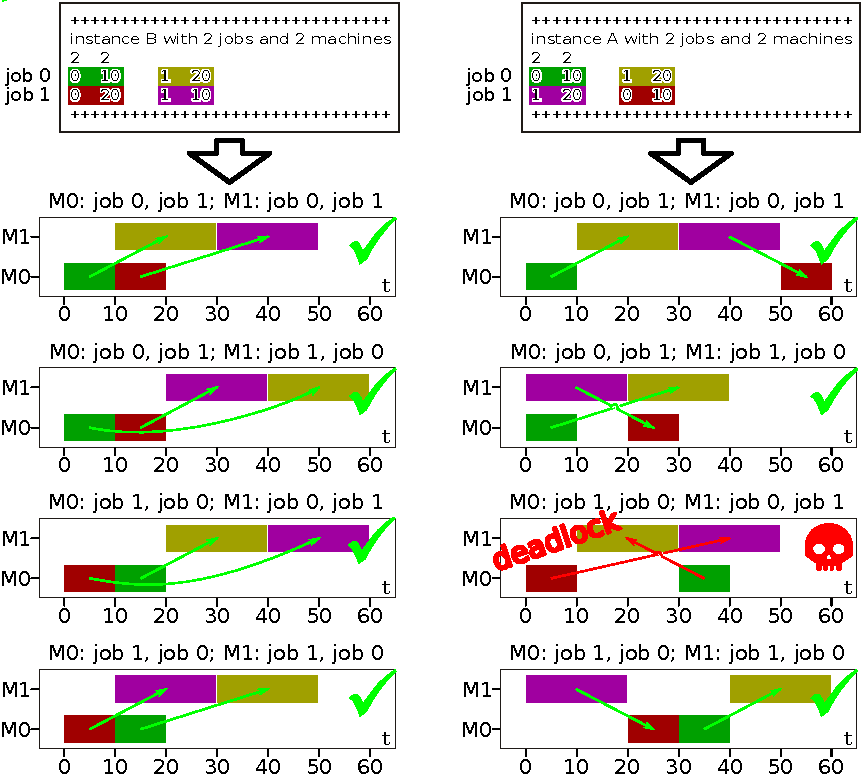
\includegraphics[width=0.85\linewidth]{\currentDir/jssp_feasible_gantt.pdf}%
\caption{Two different JSSP instances with $\jsspMachines=2$~machines and $\jsspJobs=2$~jobs.%
The left one has four feasible corresponding Gantt charts.
The right one has only three feasible solutions and one infeasible one.}%
\label{fig:jssp_feasible_gantt}%
\end{figure}%

The third schedule in the right column of \autoref{fig:jssp_feasible_gantt} illustrates exactly this case.
Machine~0 should begin by doing job~1.
Job~1 can only start on machine~0 after it has been finished on machine~1.
At machine~1, we should begin with job~0.
Before job~0 can be put on machine~1, it must go through machine~0.
So job~1 cannot go to machine~0 until it has passed through machine~1, but in order to be executed on machine~1, job~0 needs to be finished there first.
Job~0 cannot begin on machine~1 until it has been passed through machine~0, but it cannot be executed there, because job~1 needs to be finished there first.
A cyclic blockage has appeared: no job can be executed on any machine if we follow this schedule.
This is called a deadlock.

No jobs overlap in the schedule.
All operations are assigned to proper machines and receive the right processing times.
Still, the schedule is infeasible, because it cannot be executed or written down without breaking the precedence constraint.

Hence, there are only three out of four possible Gantt charts that work for this problem instance.
For a problem instance where the jobs need to pass through all machines in the same sequence, however, all possible Gantt charts will work, as also illustrated in the left column of \autoref{fig:jssp_feasible_gantt}.
The number of actually feasible Gantt charts in~\solutionSpace\ thus can be different for different problem instances.

\begin{table}%
\centering%
\caption{%
The minimal number $\min\nFeasible$ of feasible solutions over all instances with specific size \jsspJobs\ and \jsspMachines\ (compare with \autoref{tbl:jsspSolutionSpaceSizeTable}).}%
\label{tbl:jsspSolutionSpaceFeasibleTable}%
\begin{tabular}{lrrrr}%
\hline%
example&\jsspJobs&\jsspMachines&$\min\nFeasible$&$\left|\solutionSpace\right|$\\%
\hline%
\autoref{fig:jssp_feasible_gantt}&2&2&3&4\\%
&2&3&4&8\\%
&2&4&5&16\\%
&2&5&6&32\\%
&3&2&22&36\\%
&3&3&63&216\\%
&3&4&147&1\dgsep296\\%
&3&5&317&7\dgsep776\\%
&4&2&244&576\\%
&4&3&1\dgsep630&13\dgsep824\\%
&4&4&7\dgsep451&331\dgsep776\\%
&5&2&4\dgsep548&14\dgsep400\\%
&5&3&91\dgsep461&1\dgsep728\dgsep000\\%
\hline%
\end{tabular}%
\end{table}%

Different \gls{JSSP} instances can have different numbers~\nFeasible\ of possible \emph{feasible} Gantt charts, even if they have the same numbers of machines and jobs.
We just saw this in \autoref{fig:jssp_feasible_gantt}.
Naturally, for a given setting of~$\jsspMachines$ and~$\jsspJobs$, we are interested in the minimum~$\min\nFeasible$ of this number, i.e., the \emph{smallest value} that~\nFeasible\ can take on over all possible instances with \jsspJobs~jobs and \jsspMachines~machines.

Now, I don't know how to compute this number in any efficient and we only want to see out of academic curiosity.
So I just enumerated all the instances for a given combination of \jsspJobs\ and ~jsspMachines.
For each instance, I enumerated all the possible Gantt charts and counted how many were feasible, i.e., computed \nFeasible\ for that instance.
After I was done with enumerating all the instances, I know the smallest value of \nFeasible, i.e., $\min\nFeasible$, for that combination of \jsspJobs\ and~\jsspMachines.
I know that there must be a better way to get this number, probably with dynamic programming, but for now, the crude method will be sufficient.
Of course, it only works for very small values of \jsspJobs\ and~\jsspMachines.

The results in \autoref{tbl:jsspSolutionSpaceFeasibleTable} show that, at least for some instances, most of the possible Gantt charts might be infeasible, as~$\min\nFeasible$ can be much smaller than~$\left|\solutionSpace\right|$.
%
\ruleOfThumb{infeasibleSolutions}{If a problem has feasibility constraints, then we often find that most of the candidate solutions are infeasible.}%
%
This is very annoying.
The potential existence of infeasible solutions means that we cannot just pick a good element from~\solutionSpace\ (according to whatever \emph{good} means), we also must be sure that it is actually \emph{feasible}.
An optimization algorithm that may sometimes return infeasible solutions will not be acceptable.%
%
\endhsection%
%
\hsection{Summary}%
%
In this section we introduced a vital component of optimization problems: The solution space~\solutionSpace.
This space contains all the possible candidate solutions~\solspel\ for the problem.
Now, we do not yet know whether a candidate solution~\solspel\ is a good or a bad solution.
In the next sections, we will learn how to decide about that.

To ground the basic concepts of~\solutionSpace\ and~\solspel\ to some practical experience, we looked again at the \gls{JSSP} as example.
We found that Gantt charts are a proper way to express solutions to this scheduling problem.
A Gantt chart basically tells which operation should be carried out by which machine at which time.
We then briefly sketched that a Gantt chart can be represented as an instance of a \codeil{class} in Python and that we can implement basic functionality for handling such classes as an instance of \codeil{Space} interface.
We can use this later on, for now it shall not be important.

What is important is that we decided to only consider Gantt charts that do not include useless waiting time.
If an operation can be executed on a machine, we will not wait uselessly but execute it right away.
While there is an infinite number of Gantt charts with arbitrary useless waiting time, the number of Gantt charts without such time is limited (\autoref{eq:jssp_solution_space_size_upper}).
However, while it is limited, it grows very quickly and, thus, $|\solutionSpace|$ is very huge, even for seemingly small instances~\instance\ (with small \jsspMachines\ and~\jsspJobs).

Moreover, we discovered that not every Gantt chart that we can draw for a given \gls{JSSP} instance is also \emph{feasible}.
Some of them have deadlocks (\ref{fig:jssp_feasible_gantt}).
Obviously, whatever we will later do to find \emph{good} Gantt charts, we must never return an infeasible one, i.e., one that cannot actually be executed.
To make matters worse, we discovered that it is entirely possible that the vast majority of Gantt charts that we could come up with for a given instance could be infeasible.

So the \gls{JSSP} is not just a problem where the number of possible solutions is far too huge to test them all, most of these solutions may also be wrong.
And the \gls{JSSP} is an \inQuotes{average citizen} in optimization.
We may often encounter similar situations, at least in terms of the size of the solution space (not all problems have feasiblity constraints).
So optimization is indeed interesting.%
\endhsection%
\endhsection%
